\documentclass{article}

\usepackage{amsmath}
\usepackage{graphicx}

\graphicspath{ {./assets/} }

\setlength\paperwidth{20.999cm}\setlength\paperheight{29.699cm}\setlength\voffset{-1in}\setlength\hoffset{-1in}\setlength\topmargin{1.499cm}\setlength\headheight{12pt}\setlength\headsep{0cm}\setlength\footskip{1.131cm}\setlength\textheight{25cm}\setlength\oddsidemargin{2.499cm}\setlength\textwidth{15.999cm}

\begin{document}
\begin{center}
\hrule

\vspace{.4cm}
{\bf {\Huge Assignment 4}} \\
\vspace{.2cm}
{\bf Computer Graphics}
\vspace{.2cm}
\end{center}{\bf Edoardo Riggio } (edoardo.riggio@usi.ch) \hspace{\fill}  \today \\
\hrule
\vspace{.2cm}

\section{Exercise 1}
\subsection{Task 1}
The two matrices $R_{90}$ and $T$ in homogeneous coordinates are as follows.
\[ R_{90} = \begin{bmatrix} 1 & 0 & 1 \\ 0 & 1 & -2 \\ 0 & 0 & 1 \end{bmatrix} \]
\[ T = \begin{bmatrix} \cos{90} & -\sin{90} & 0 \\ \sin{90} & \cos{90} & 0 \\ 0 & 0 & 1 \end{bmatrix} = \begin{bmatrix} 0 & -1 & 0 \\ 1 & 0 & 0 \\ 0 & 0 & 1 \end{bmatrix} \]

\subsection{Task 2}
The following are the computations for the rotated and translated points and vector.
\begin{align*}
	p'_1 & =  \begin{bmatrix}1&0&1\\ 0&1&-2\\0&0&1\end{bmatrix} \left( \begin{bmatrix}0&-1&0\\ 1&0&0\\ 0&0&1\end{bmatrix}\begin{bmatrix}1\\ 1\\ 1\end{bmatrix} \right)  =  \begin{bmatrix}1&0&1\\ 0&1&-2\\0&0&1\end{bmatrix}\begin{bmatrix}0\cdot 1+\left(-1\right)\cdot 1+0\cdot 1\\ 1\cdot 1+0\cdot 1+0\cdot 1\\ 0\cdot 1+0\cdot 1+1\cdot 1\end{bmatrix} \\
	& = \begin{bmatrix}1&0&1\\ 0&1&-2\\0&0&1\end{bmatrix}\begin{bmatrix}-1\\ 1\\ 1\end{bmatrix} = \begin{bmatrix}1\cdot \left(-1\right)+0\cdot 1+1\cdot 1\\ 0\cdot \left(-1\right)+1\cdot 1+\left(-2\right)\cdot 1\\ 0\cdot \left(-1\right)+0\cdot 1+1\cdot 1\end{bmatrix} = \begin{bmatrix}0\\ -1\\ 1\end{bmatrix} \mapsto \begin{bmatrix}0\\ -1\end{bmatrix}
\end{align*}

\begin{align*}
	p'_2 & =  \begin{bmatrix}1&0&1\\ 0&1&-2\\0&0&1\end{bmatrix} \left( \begin{bmatrix}0&-1&0\\ 1&0&0\\ 0&0&1\end{bmatrix}\begin{bmatrix}3\\ 2\\ 1\end{bmatrix} \right)  =  \begin{bmatrix}1&0&1\\ 0&1&-2\\0&0&1\end{bmatrix}\begin{bmatrix}0\cdot 3+\left(-1\right)\cdot 2+0\cdot 1\\ 1\cdot 3+0\cdot 2+0\cdot 1\\ 0\cdot 3+0\cdot 2+1\cdot 1\end{bmatrix} \\
	& = \begin{bmatrix}1&0&1\\ 0&1&-2\\0&0&1\end{bmatrix}\begin{bmatrix}-2\\ 3\\ 1\end{bmatrix} = \begin{bmatrix}1\cdot \left(-2\right)+0\cdot 3+1\cdot 1\\ 0\cdot \left(-2\right)+1\cdot 3+\left(-2\right)\cdot 1\\ 0\cdot \left(-2\right)+0\cdot 3+1\cdot 1\end{bmatrix} = \begin{bmatrix}-1\\ 1\\ 1\end{bmatrix} \mapsto \begin{bmatrix}-1\\ 1\end{bmatrix}
\end{align*}

\begin{align*}
	p'_2 & =  \begin{bmatrix}1&0&1\\ 0&1&-2\\0&0&1\end{bmatrix} \left( \begin{bmatrix}0&-1&0\\ 1&0&0\\ 0&0&1\end{bmatrix}\begin{bmatrix}1\\ 4\\ 1\end{bmatrix} \right)  =  \begin{bmatrix}1&0&1\\ 0&1&-2\\0&0&1\end{bmatrix}\begin{bmatrix}0\cdot 1+\left(-1\right)\cdot 4+0\cdot 1\\ 1\cdot 1+0\cdot 4+0\cdot 1\\ 0\cdot 1+0\cdot 4+1\cdot 1\end{bmatrix} \\
	& = \begin{bmatrix}1&0&1\\ 0&1&-2\\0&0&1\end{bmatrix}\begin{bmatrix}-4\\ 1\\ 1\end{bmatrix} = \begin{bmatrix}1\cdot \left(-4\right)+0\cdot 1+1\cdot 1\\ 0\cdot \left(-4\right)+1\cdot 1+\left(-2\right)\cdot 1\\ 0\cdot \left(-4\right)+0\cdot 1+1\cdot 1\end{bmatrix} = \begin{bmatrix}-3\\ -1\\ 1\end{bmatrix} \mapsto \begin{bmatrix}-3\\ -1\end{bmatrix}
\end{align*}

\begin{align*}
	p' & =  \begin{bmatrix}1&0&1\\ 0&1&-2\\0&0&1\end{bmatrix} \left( \begin{bmatrix}0&-1&0\\ 1&0&0\\ 0&0&1\end{bmatrix}\begin{bmatrix}1.5\\ 2.5\\ 1\end{bmatrix} \right)  =  \begin{bmatrix}1&0&1\\ 0&1&-2\\0&0&1\end{bmatrix}\begin{bmatrix}0\cdot 1.5+\left(-1\right)\cdot 2.5+0\cdot 1\\ 1\cdot 1.5+0\cdot 2.5+0\cdot 1\\ 0\cdot 1.5+0\cdot 2.5+1\cdot 1\end{bmatrix} \\
	& = \begin{bmatrix}1&0&1\\ 0&1&-2\\0&0&1\end{bmatrix}\begin{bmatrix}-2.5\\ 1.5\\ 1\end{bmatrix} = \begin{bmatrix}1\cdot \left(-2.5\right)+0\cdot 1.5+1\cdot 1\\ 0\cdot \left(-2.5\right)+1\cdot 1.5+\left(-2\right)\cdot 1\\ 0\cdot \left(-2.5\right)+0\cdot 1.5+1\cdot 1\end{bmatrix} = \begin{bmatrix}-1.5\\ -0.5\\ 1\end{bmatrix} \mapsto \begin{bmatrix}-1.5\\ -0.5 \end{bmatrix}
\end{align*}

\begin{align*}
	u' & =  \begin{bmatrix}1&0&1\\ 0&1&-2\\0&0&1\end{bmatrix} \left( \begin{bmatrix}0&-1&0\\ 1&0&0\\ 0&0&1\end{bmatrix}\begin{bmatrix}0.5\\ 1.5\\ 0\end{bmatrix} \right)  =  \begin{bmatrix}1&0&1\\ 0&1&-2\\0&0&1\end{bmatrix}\begin{bmatrix}0\cdot 0.5+\left(-1\right)\cdot 1.5+0\cdot 0\\ 1\cdot 0.5+0\cdot 1.5+0\cdot 0\\ 0\cdot 0.5+0\cdot 1.5+1\cdot 0\end{bmatrix} \\
	& = \begin{bmatrix}1&0&1\\ 0&1&-2\\0&0&1\end{bmatrix}\begin{bmatrix}-1.5\\ 0.5\\ 0\end{bmatrix} = \begin{bmatrix}1\cdot \left(-1.5\right)+0\cdot 0.5+1\cdot 0\\ 0\cdot \left(-1.5\right)+1\cdot 0.5+\left(-2\right)\cdot 0\\ 0\cdot \left(-1.5\right)+0\cdot 0.5+1\cdot 0\end{bmatrix} = \begin{bmatrix}-1.5\\ 0.5\\ 0\end{bmatrix} \mapsto \begin{bmatrix}-1.5\\ 0.5 \end{bmatrix}
\end{align*}
Now we can see that $u' = p' - p'_1$, as shown below:
\[ \begin{bmatrix}-1.5\\ 0.5\\ 0\end{bmatrix} = \begin{bmatrix}-1.5\\ -0.5\\ 1\end{bmatrix} - \begin{bmatrix}0\\ -1\\ 1\end{bmatrix} = \begin{bmatrix}-1.5\\ 0.5\\ 0\end{bmatrix} \]
The translation only works with points, while the rotation works with both points and vectors. For this reason, the vector $u'$ is only affected by the rotation matrix, and not by the translation matrix. \\ \\
Finally, here is a visual representation of all the points and vector before and after the transformations. \\

\begin{center}
	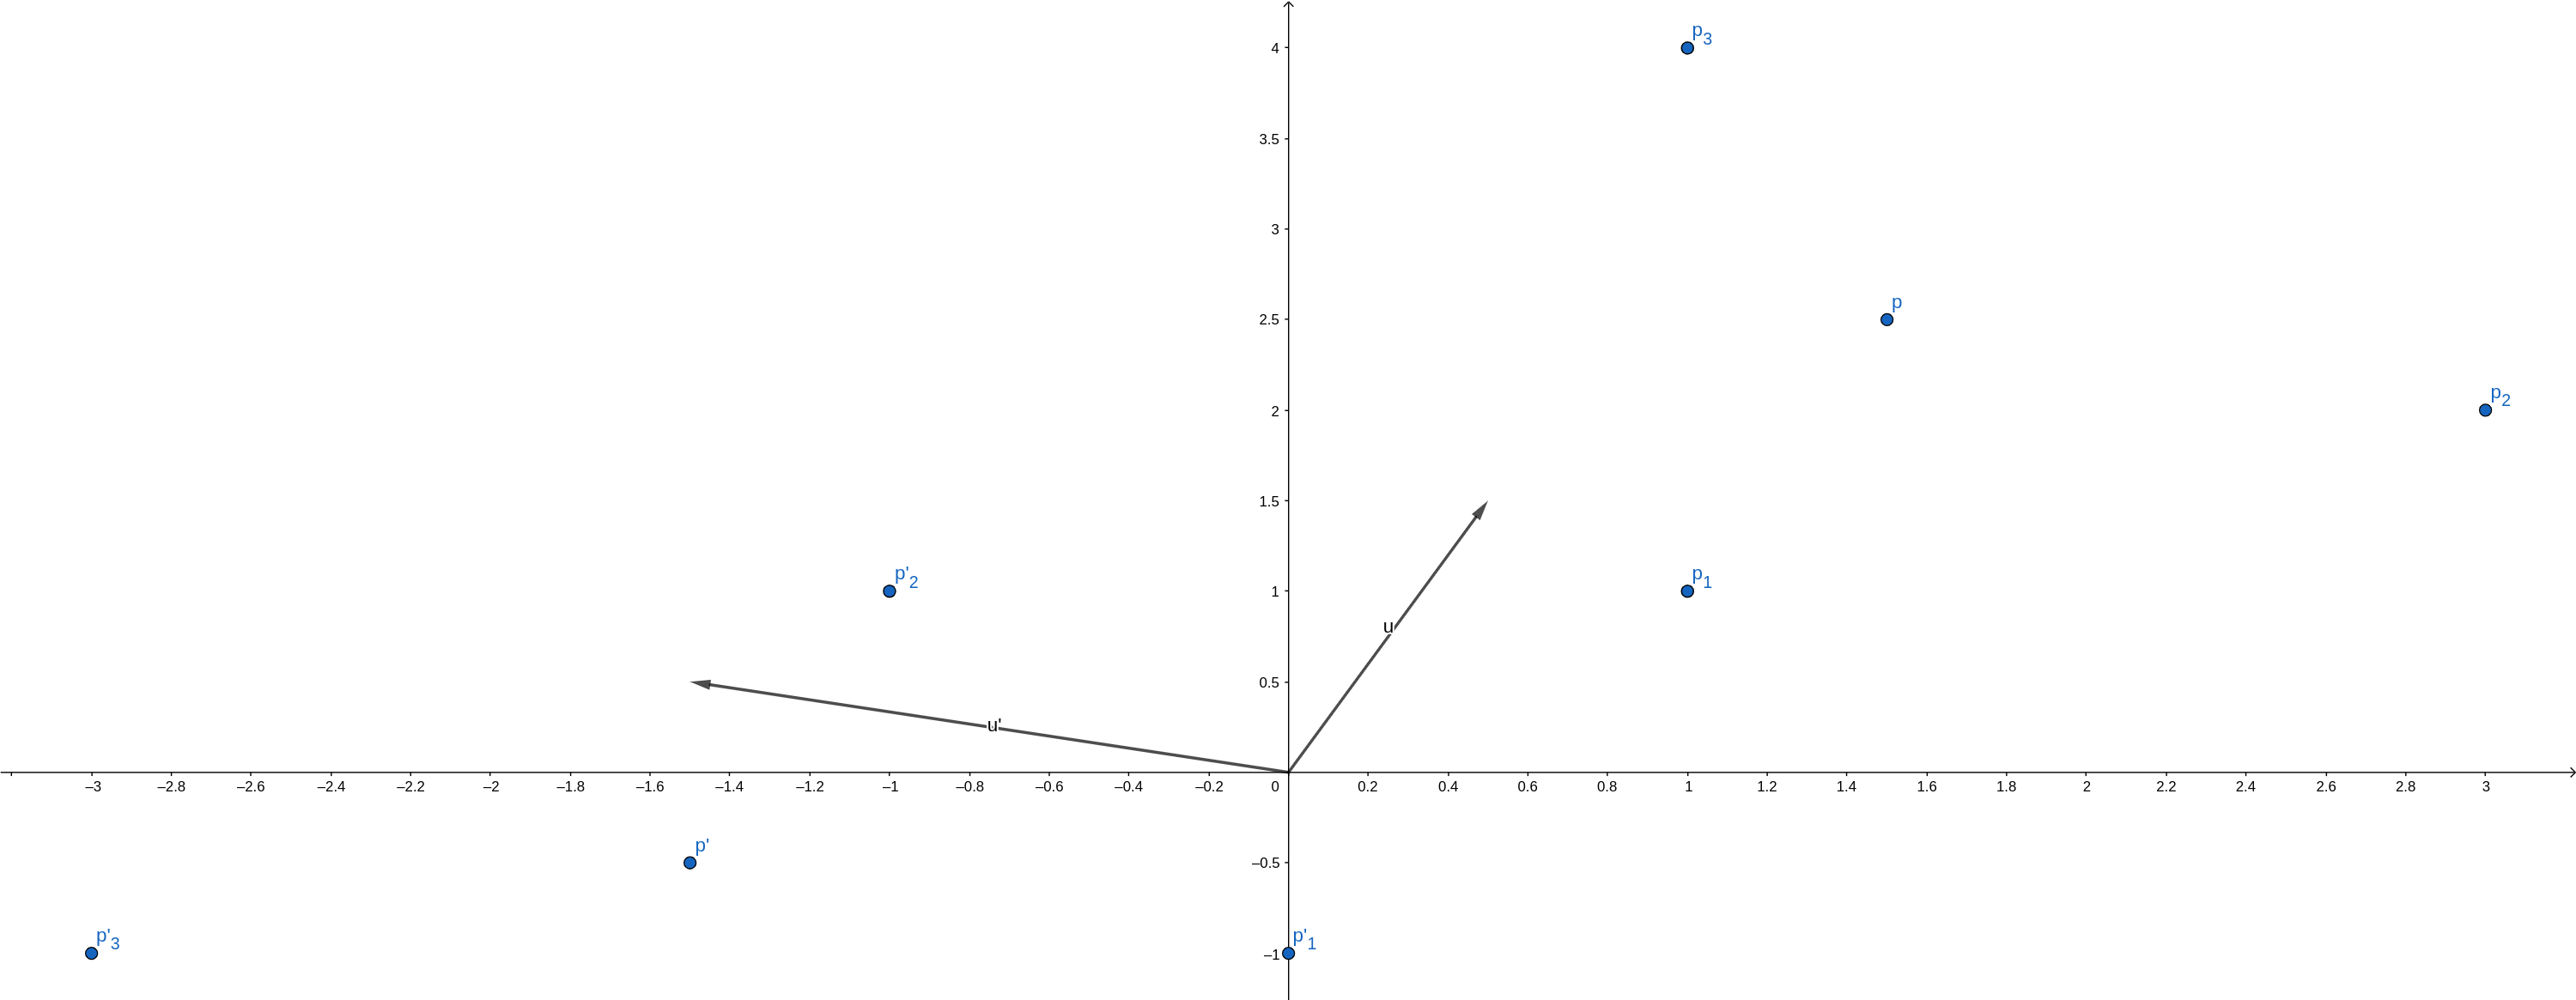
\includegraphics[width=15cm]{task_2.png}
\end{center}

\subsection{Task 3}
Here we have the scaling matrix which scales both $x$ and $y$ by a factor of 2.
\[ S = \begin{bmatrix} 2 & 0 & 0 \\ 0 & 2 & 0 \\ 0 & 0 & 1 \end{bmatrix} \]
The following are the computations for the scaled points and vector.

\begin{align*}
	p''_1 = \begin{bmatrix}2&0&0\\ 0&2&0\\ 0&0&1\end{bmatrix}\begin{bmatrix}0\\ -1\\ 1\end{bmatrix} = \begin{bmatrix}2\cdot 0+0\cdot \left(-1\right)+0\cdot 1\\ 0\cdot 0+2\left(-1\right)+0\cdot 1\\ 0\cdot 0+0\cdot \left(-1\right)+1\cdot 1\end{bmatrix} = \begin{bmatrix}0\\ -2\\ 1\end{bmatrix} \mapsto \begin{bmatrix}0\\ -2\end{bmatrix}
\end{align*}

\begin{align*}
	p''_2 = \begin{bmatrix}2&0&0\\ 0&2&0\\ 0&0&1\end{bmatrix}\begin{bmatrix}-1\\ 1\\ 1\end{bmatrix} = \begin{bmatrix}2\left(-1\right)+0\cdot 1+0\cdot 1\\ 0\cdot \left(-1\right)+2\cdot 1+0\cdot 1\\ 0\cdot \left(-1\right)+0\cdot 1+1\cdot 1\end{bmatrix} = \begin{bmatrix}-2\\ 2\\ 1\end{bmatrix} \mapsto \begin{bmatrix}-2\\ 2\end{bmatrix}
\end{align*}

\begin{align*}
	p''_3 = \begin{bmatrix}2&0&0\\ 0&2&0\\ 0&0&1\end{bmatrix}\begin{bmatrix}-3\\ -1\\ 1\end{bmatrix} = \begin{bmatrix}2\left(-3\right)+0\cdot \left(-1\right)+0\cdot 1\\ 0\cdot \left(-3\right)+2\left(-1\right)+0\cdot 1\\ 0\cdot \left(-3\right)+0\cdot \left(-1\right)+1\cdot 1\end{bmatrix} = \begin{bmatrix}-6\\ -2\\ 1\end{bmatrix} \mapsto \begin{bmatrix}-6\\ -2\end{bmatrix}
\end{align*}

\begin{align*}
	p'' = \begin{bmatrix}2&0&0\\ 0&2&0\\ 0&0&1\end{bmatrix}\begin{bmatrix}-1.5\\ -0.5\\ 1\end{bmatrix} = \begin{bmatrix}2\left(-1.5\right)+0\cdot \left(-0.5\right)+0\cdot 1\\ 0\cdot \left(-1.5\right)+2\left(-0.5\right)+0\cdot 1\\ 0\cdot \left(-1.5\right)+0\cdot \left(-0.5\right)+1\cdot 1\end{bmatrix} = \begin{bmatrix}-3\\ -1\\ 1\end{bmatrix} \mapsto \begin{bmatrix}-3\\ -1\end{bmatrix}
\end{align*}

\begin{align*}
	u'' = \begin{bmatrix}2&0&0\\ 0&2&0\\ 0&0&1\end{bmatrix}\begin{bmatrix}-1.5\\ 0.5\\ 0\end{bmatrix} = \begin{bmatrix}2\left(-1.5\right)+0\cdot 0.5+0\cdot 0\\ 0\cdot \left(-1.5\right)+2\cdot 0.5+0\cdot 0\\ 0\cdot \left(-1.5\right)+0\cdot 0.5+1\cdot 0\end{bmatrix} = \begin{bmatrix}-3\\ 1\\ 0\end{bmatrix} \mapsto \begin{bmatrix}-3\\ 1\end{bmatrix}
\end{align*}
Finally, here is a visual representation of the points and the vector before and after the scaling. \\

\begin{center}
	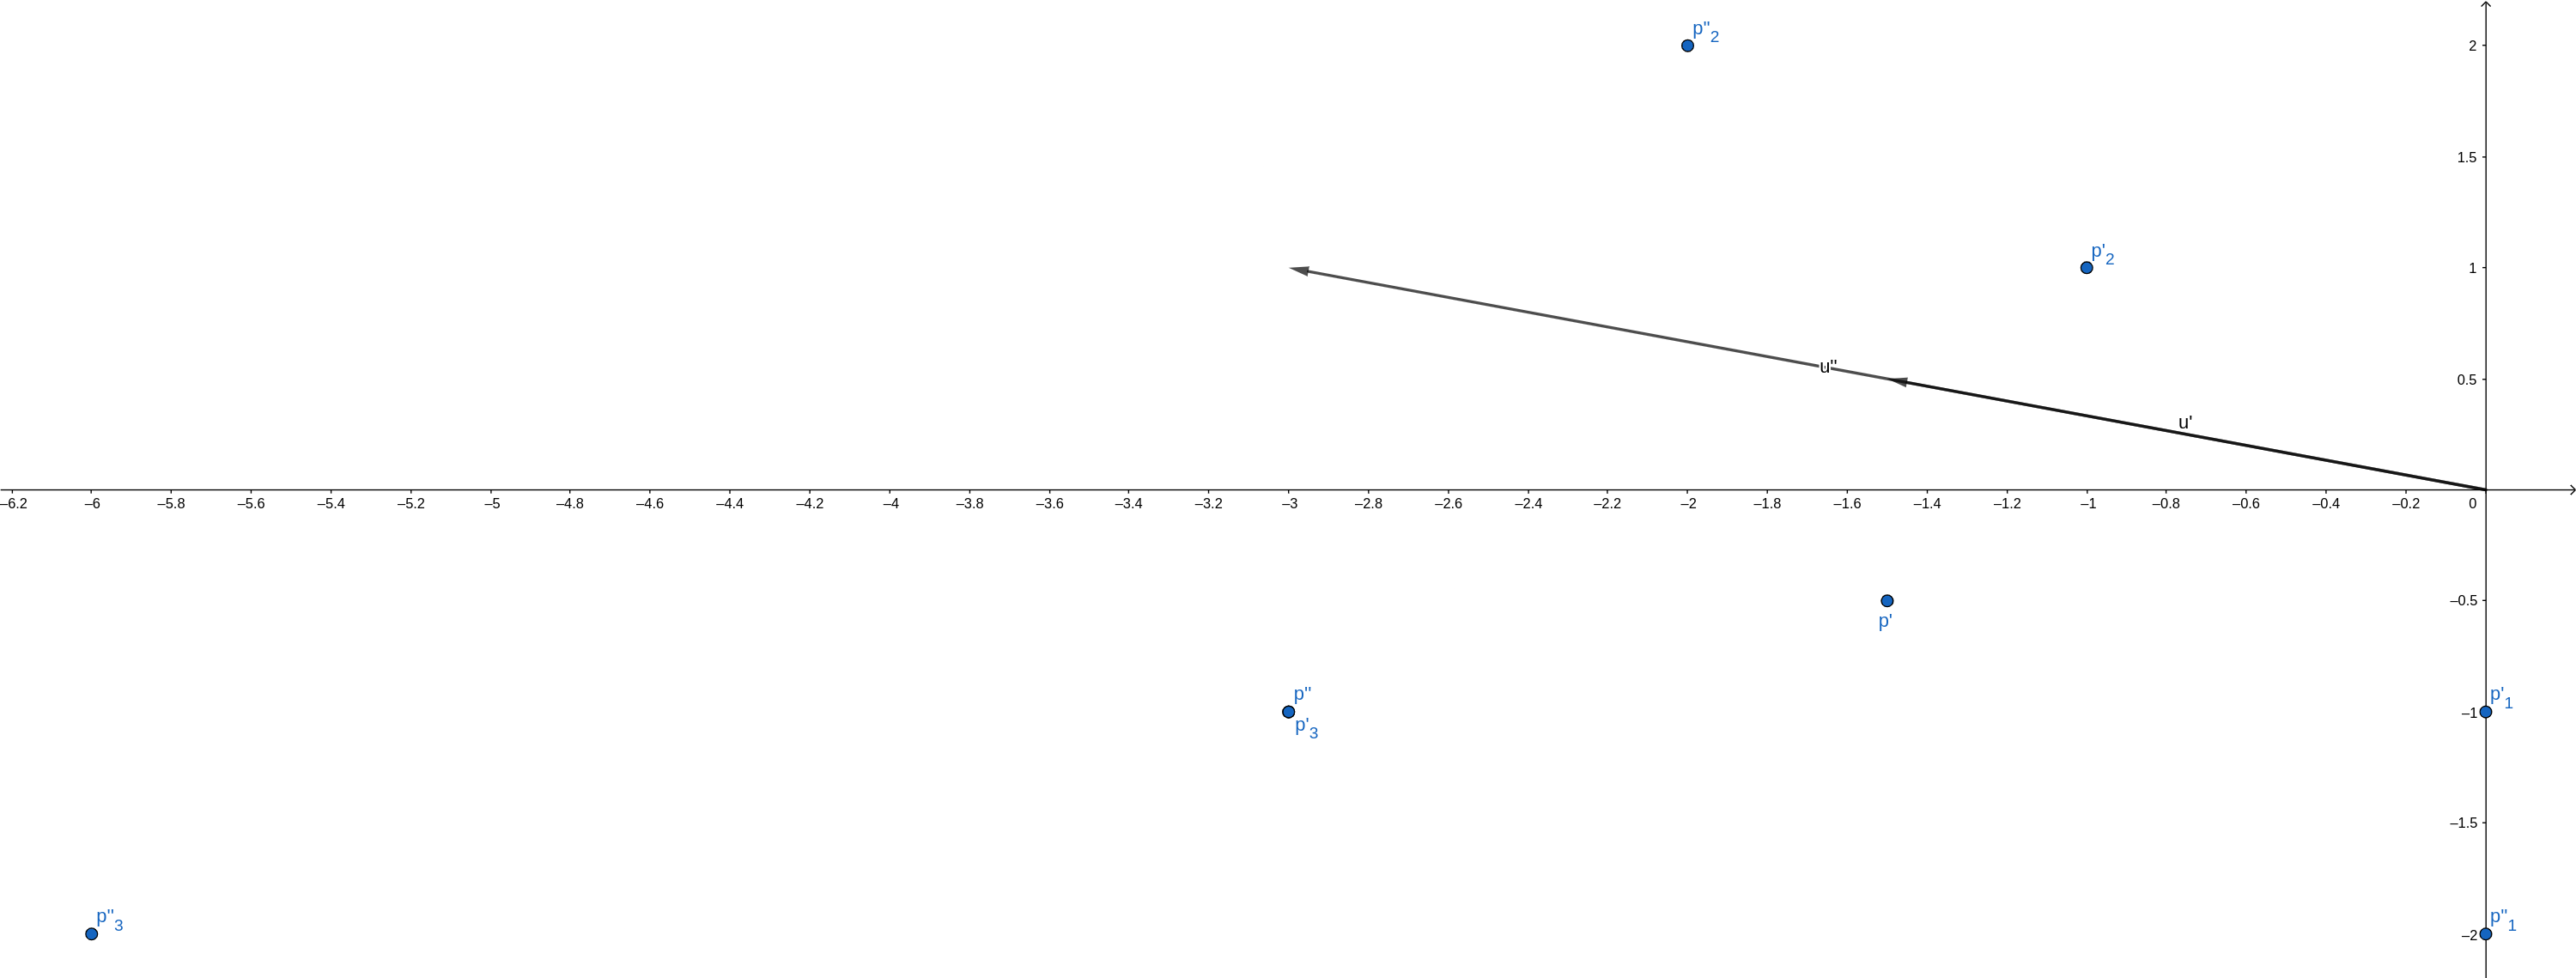
\includegraphics[width=15cm]{task_3.png}
\end{center}

\subsection{Task 4}
In order to apply the inverse transformations, we need to compute the inverse matrices for rotation, translation and scaling.
\[ R_{90}^{-1} = \begin{bmatrix} 0 & 1 & 0 \\ -1 & 0 & 0 \\ 0 & 0 & 1 \end{bmatrix} \]
\[ T^{-1} = \begin{bmatrix} 1 & 0 & -1 \\ 0 & 1 & 2 \\ 0 & 0 & 1 \end{bmatrix} \]
\[ S^{-1} = \begin{bmatrix} 0.5 & 0 & 0 \\ 0 & 0.5 & 0 \\ 0 & 0 & 1 \end{bmatrix} \]
And we compute the transformation matrix $M$.

\begin{align*}
	M & = R_{90}^{-1} T^{-1} S^{-1} = \begin{bmatrix} 0 & 1 & 0 \\ -1 & 0 & 0 \\ 0 & 0 & 1 \end{bmatrix} \begin{bmatrix} 1 & 0 & -1 \\ 0 & 1 & 2 \\ 0 & 0 & 1 \end{bmatrix} \begin{bmatrix} 0.5 & 0 & 0 \\ 0 & 0.5 & 0 \\ 0 & 0 & 1 \end{bmatrix} \\ 
	& = \begin{bmatrix}0\cdot 1+1\cdot 0+0\cdot 0&0\cdot 0+1\cdot 1+0\cdot 0&0\cdot \left(-1\right)+1\cdot 2+0\cdot 1\\ \left(-1\right)\cdot 1+0\cdot 0+0\cdot 0&\left(-1\right)\cdot 0+0\cdot 1+0\cdot 0&\left(-1\right)\left(-1\right)+0\cdot 2+0\cdot 1\\ 0\cdot 1+0\cdot 0+1\cdot 0&0\cdot 0+0\cdot 1+1\cdot 0&0\cdot \left(-1\right)+0\cdot 2+1\cdot 1\end{bmatrix} \begin{bmatrix} 0.5 & 0 & 0 \\ 0 & 0.5 & 0 \\ 0 & 0 & 1 \end{bmatrix} \\
	& = \begin{bmatrix}0&1&2\\ -1&0&1\\ 0&0&1\end{bmatrix} \begin{bmatrix} 0.5 & 0 & 0 \\ 0 & 0.5 & 0 \\ 0 & 0 & 1 \end{bmatrix} \\
	& = \begin{bmatrix}0\cdot 0.5+1\cdot 0+2\cdot 0&0\cdot 0+1\cdot 0.5+2\cdot 0&0\cdot 0+1\cdot 0+2\cdot 1\\ \left(-1\right)\cdot 0.5+0\cdot 0+1\cdot 0&\left(-1\right)\cdot 0+0\cdot 0.5+1\cdot 0&\left(-1\right)\cdot 0+0\cdot 0+1\cdot 1\\ 0\cdot 0.5+0\cdot 0+1\cdot 0&0\cdot 0+0\cdot 0.5+1\cdot 0&0\cdot 0+0\cdot 0+1\cdot 1\end{bmatrix} = \begin{bmatrix}0&0.5&2\\ -0.5&0&1\\ 0&0&1\end{bmatrix}
\end{align*}

\pagebreak
\noindent Now that we have the transformation matrix $M$, we can finally compute the transformation of points $p_1''$, $p_2''$, $p_3''$, $p''$ and of vector $u''$.

\begin{align*}
	p_1 & = \begin{bmatrix}0&0.5&2\\ -0.5&0&1\\ 0&0&1\end{bmatrix} \begin{bmatrix}0\\ -2\\ 1\end{bmatrix} = \begin{bmatrix}0\cdot 0+0.5\left(-2\right)+2\cdot 1\\ \left(-0.5\right)\cdot 0+0\cdot \left(-2\right)+1\cdot 1\\ 0\cdot 0+0\cdot \left(-2\right)+1\cdot 1\end{bmatrix} = \begin{bmatrix}1\\ 1\\ 1\end{bmatrix}
\end{align*}

\begin{align*}
	p_2 & = \begin{bmatrix}0&0.5&2\\ -0.5&0&1\\ 0&0&1\end{bmatrix} \begin{bmatrix}-2\\ 2\\ 1\end{bmatrix} = \begin{bmatrix}0\cdot \left(-2\right)+0.5\cdot 2+2\cdot 1\\ \left(-0.5\right)\left(-2\right)+0\cdot 2+1\cdot 1\\ 0\cdot \left(-2\right)+0\cdot 2+1\cdot 1\end{bmatrix} = \begin{bmatrix}3\\ 2\\ 1\end{bmatrix}
\end{align*}

\begin{align*}
	p_2 & = \begin{bmatrix}0&0.5&2\\ -0.5&0&1\\ 0&0&1\end{bmatrix} \begin{bmatrix}-6\\ -2\\ 1\end{bmatrix} = \begin{bmatrix}0\cdot \left(-6\right)+0.5\left(-2\right)+2\cdot 1\\ \left(-0.5\right)\left(-6\right)+0\cdot \left(-2\right)+1\cdot 1\\ 0\cdot \left(-6\right)+0\cdot \left(-2\right)+1\cdot 1\end{bmatrix} = \begin{bmatrix}1\\ 4\\ 1\end{bmatrix}
\end{align*}

\begin{align*}
	p & = \begin{bmatrix}0&0.5&2\\ -0.5&0&1\\ 0&0&1\end{bmatrix} \begin{bmatrix}-3\\ -1\\ 1\end{bmatrix} = \begin{bmatrix}0\cdot \left(-3\right)+0.5\left(-1\right)+2\cdot 1\\ \left(-0.5\right)\left(-3\right)+0\cdot \left(-1\right)+1\cdot 1\\ 0\cdot \left(-3\right)+0\cdot \left(-1\right)+1\cdot 1\end{bmatrix} = \begin{bmatrix}1.5\\ 2.5\\ 1\end{bmatrix}
\end{align*}

\begin{align*}
	u & = \begin{bmatrix}0&0.5&2\\ -0.5&0&1\\ 0&0&1\end{bmatrix} \begin{bmatrix}-3\\ 1\\ 0\end{bmatrix} = \begin{bmatrix}0\cdot \left(-3\right)+0.5\cdot 1+2\cdot 0\\ \left(-0.5\right)\left(-3\right)+0\cdot 1+1\cdot 0\\ 0\cdot \left(-3\right)+0\cdot 1+1\cdot 0\end{bmatrix} = \begin{bmatrix}0.5\\ 1.5\\ 0\end{bmatrix}
\end{align*}
As we can see, by multiplying the transformation matrix with $p_1''$, $p_2''$, $p_3''$, $p''$ and $u''$, we will get back $p_1$, $p_2$, $p_3$, $p$ and $u$.

\subsection{Task 5}
First we need to compute the barycentric coordinates of point $p$ with respect to the triangle made up by the points $p_1$, $p_2$ and $p_3$. To do so we use the following system of linear equations.
\begin{align*}
	\begin{cases} x = x_1 + \lambda_2 (x_2-x_1) + \lambda_3 (x_3-x_1) \\ y = y_1 + \lambda_2 (y_2-y_1) + \lambda_3 (y_3-y_1) \end{cases}
\end{align*}
And compute $\lambda_1$ as follows.
\[ \lambda_1 = 1 - \lambda_2 - \lambda_3 \]
Now we compute the actual values.
\begin{align*}
	& \begin{cases} 1.5 = 1 + \lambda_2(3-1) + \lambda_3(1-1) \\ 2.5 = 1 + \lambda_2(2-1) + \lambda_3(4-1) \end{cases} \\ 
	& \begin{cases} 1.5 = 1+2 \lambda_2 \\ 2.5 = 1 + \lambda_2 + 3 \lambda_3 \end{cases} \\ 
	& \begin{cases} -2\lambda_2 = -1.5+1 \\ -3\lambda_3 = -2.5+1+\lambda_2 \end{cases} \\
	& \begin{cases} -2\lambda_2 = -0.5 \\ -3\lambda_3 = -2.5+1+\lambda_2 \end{cases} \\
	& \begin{cases} \lambda_2 = \displaystyle \frac{0.5}{2} \\ 3\lambda_3 = 2.5-1-\lambda_2 \end{cases} \\
	& \begin{cases} \lambda_2 = 0.25 \\ \lambda_3 = \displaystyle \frac{2.5 - 1 - 0.25}{3}  \end{cases} \\
	& \begin{cases} \lambda_2 = 0.25 \\ \lambda_3 = 0.42 \end{cases}
\end{align*}
\begin{align*}
	\lambda_1 = 1 - 0.25 - 0.42 = 0.33
\end{align*}
Thus we have the following values for the lambdas.
\[ \lambda_1 = \displaystyle \frac{1}{3} \]
\[ \lambda_2 = \displaystyle \frac{1}{4} \]
\[ \lambda_3 = \displaystyle \frac{5}{12} \]
Now we compute the barycentric coordinates of point $p''$ with respect to the triangle made up by the points $p_1''$, $p_2''$ and $p_3''$. To do so we use the following system of linear equations.
\begin{align*}
	\begin{cases} x = x_1 + \lambda_2 (x_2-x_1) + \lambda_3 (x_3-x_1) \\ y = y_1 + \lambda_2 (y_2-y_1) + \lambda_3 (y_3-y_1) \end{cases}
\end{align*}
And compute $\lambda_1$ as follows.
\[ \lambda_1 = 1 - \lambda_2 - \lambda_3 \]
Now we compute the actual values.
\begin{align*}
	& \begin{cases} -3 = \lambda_2(-2-0) + \lambda_3(-6-0) \\ -1 = -2 + \lambda_2(2+2) + \lambda_3(-2+2) \end{cases} \\ 
	& \begin{cases} -3 = -2 \lambda_2 -6 \lambda_3 \\ -1 = -2 +4 \lambda_2 \end{cases} \\ 
	& \begin{cases} 6\lambda_3 = 3 - 2\lambda_2 \\ -4\lambda_2 = 1-2 \end{cases} \\
	& \begin{cases} 6\lambda_3 = 3 - 2\lambda_2 \\ 4\lambda_2 = 1 \end{cases} \\
	& \begin{cases} 6\lambda_3 = 2.5 \\ \lambda_2 = \displaystyle \frac{1}{4} \end{cases} \\
	& \begin{cases} \lambda_3 = \displaystyle \frac{2.5}{6} \\ \lambda_2 = 0.25  \end{cases} \\
	& \begin{cases} \lambda_3 = 0.42 \\ \lambda_2 = 0.25 \end{cases}
\end{align*}
\begin{align*}
	\lambda_1 = 1 - 0.25 - 0.42 = 0.33
\end{align*}

Thus we have the following values for the lambdas.
\[ \lambda_1 = \displaystyle \frac{1}{3} \]
\[ \lambda_2 = \displaystyle \frac{1}{4} \]
\[ \lambda_3 = \displaystyle \frac{5}{12} \]
As expected, the barycentric coordinates to not change. This is because together with points $p_1$, $p_2$ and $p_3$, also $p$ undergoes the same kind of transformation. This means that $p''$ will be in the same position relative to $p_1''$, $p_2''$ and $p_3''$ as it was $p$ for $p_1$, $p_2$ and $p_3$.

\section{Exercise 2}
In order to project the points $p_i$ onto the line $x = 1$, we need to use the following matrix.
\[ M = \begin{bmatrix} 1 & 0 & 0 \\ 0 & 1 & 0 \\ 1 & 0 & 0 \end{bmatrix} \]
This is because if we multiply a random point of the form:
\[ p = \begin{bmatrix} x \\ y \\ 1 \end{bmatrix} \]
We will obtain the following.
\[ \begin{bmatrix} 1 & 0 & 0 \\ 0 & 1 & 0 \\ 1 & 0 & 0 \end{bmatrix} \begin{bmatrix} x \\ y \\ 1 \end{bmatrix} = \begin{bmatrix} x \\ y \\ x \end{bmatrix} \]
And finally, in order to obtain the homogeneous coordinates of the point -- and transform them into cartesian coordinates, we need to divide every term of the matrix by $x$. This is because the third term of the matrix is a $x$. The computation is as follows.
\[ \begin{bmatrix} x/x \\ y/x \\ x/x \end{bmatrix} = \begin{bmatrix} 1 \\ y/x \\ 1 \end{bmatrix} \mapsto \begin{bmatrix} 1 \\ y/x \end{bmatrix}  \]

\section{Exercise 3}
In order to project any point $p_i$ onto the general line $y = ax + b$, we need to use the following matrix.
\[ M = \begin{bmatrix} b & 0 & 0 \\ 0 & b & 0 \\ -a & 1 & 0 \end{bmatrix} \]
This matrix comes from the solution of the system of linear equations composed by:
\[ y' = \frac{y}{x} x' \]
And
\[ y' = ax'+b \]
First of all we substitute the $y'$ of the second equation in the first equation.
\begin{align*}
	\frac{y}{x} x' & = ax' + b \\
	b & = \frac{y}{x} x' - ax' \\
	b & = x' \left( \frac{y}{x} - a \right) \\
	x' & = \frac{b}{\frac{y}{x} - a}
\end{align*}
Next we substitute the $x'$ we just found into the second equation.
\begin{align*}
	y' & = a \left( \frac{b}{\frac{y}{x}-a} \right) + b \\
	y' & = \frac{ab}{\frac{y}{x}-a} + b \\
	y' & = \frac{ab + \frac{by}{x} -ba}{\frac{y}{x}-a} \\
	y' & = \frac{ \frac{by}{x}}{\frac{y}{x}-a}
\end{align*}
Now that we found the equations for both $x'$ and $y'$, we need to find the matrix that allows for this transformation.
\begin{align*}
	\begin{bmatrix} x' \\ y' \\ 1 \end{bmatrix} = \begin{bmatrix} \frac{b}{\frac{y}{x} - a} \\  \frac{ \frac{by}{x}}{\frac{y}{x}-a} \\ 1 \end{bmatrix} = \begin{bmatrix} b \\  \frac{by}{x} \\ \frac{y}{x}-a \end{bmatrix} = \begin{bmatrix} b \\  by \\ y-ax \end{bmatrix}
\end{align*}
In the above formula I've multiplied the three terms by $\frac{y}{x} - a$ and by $x$, since divisions cannot be translated in the matrix $M$. Finally we obtain the following.
\[ \begin{bmatrix} b & 0 & 0 \\ 0 & b & 0 \\ -a & 1 & 0 \end{bmatrix} \begin{bmatrix} x \\ y \\ 1 \end{bmatrix} = \begin{bmatrix} b \\  by \\ y-ax \end{bmatrix} \]
Thus making $M$ the correct matrix used to compute the point $p_i'$. In order to obtain the cartesian coordinates of the point, we need to divide all of the three terms by $y - ax$, thus obtaining:
\[ \begin{bmatrix} \frac{b}{y-ax} \\  \frac{by}{y-ax} \\ \frac{y-ax}{y-ax} \end{bmatrix} = \begin{bmatrix} \frac{b}{y-ax} \\ \frac{by}{y-ax} \\ 1 \end{bmatrix} \mapsto \begin{bmatrix} \frac{b}{y-ax} \\ \frac{by}{y-ax} \end{bmatrix} \]

\end{document}


















